%!TEX root = ../thesis.tex
%*******************************************************************************
%*********************************** First Chapter *****************************
%*******************************************************************************

\chapter{Introduction}  %Title of the First Chapter

\ifpdf
    \graphicspath{{Chapter1/Figs/Raster/}{Chapter1/Figs/PDF/}{Chapter1/Figs/}}
\else
    \graphicspath{{Chapter1/Figs/Vector/}{Chapter1/Figs/}}
\fi


\section{Introduction to epigenetics in prokaryotes, animals, and plants } %Section - 1.1 

Epigenetics can be described as “a stably heritable phenotype resulting from changes in a chromosome without alterations in the DNA sequence” \citep{RN135}. The addition of a methyl group to the 5th carbon of cytosine results 5-methyl-cytosine and a pattern of DNA methylation. This is the most prominent form of DNA methylation in plants and occurs predominantly in heterochromatic regions, however, there also exist methylated loci in genic regions. In prokaryotic organisms, DNA methylation was originally identified as a component in the restriction-modification (R-M) pathway whereby methylated sequences are identified as self and unmethylated sequences are targeted for cleavage by restriction enzymes, thus protecting the integrity of the genome from invading unmetylated phage DNA  \citep{RN96,RN95}.

\begin{figure}[htbp!] 
\centering    
    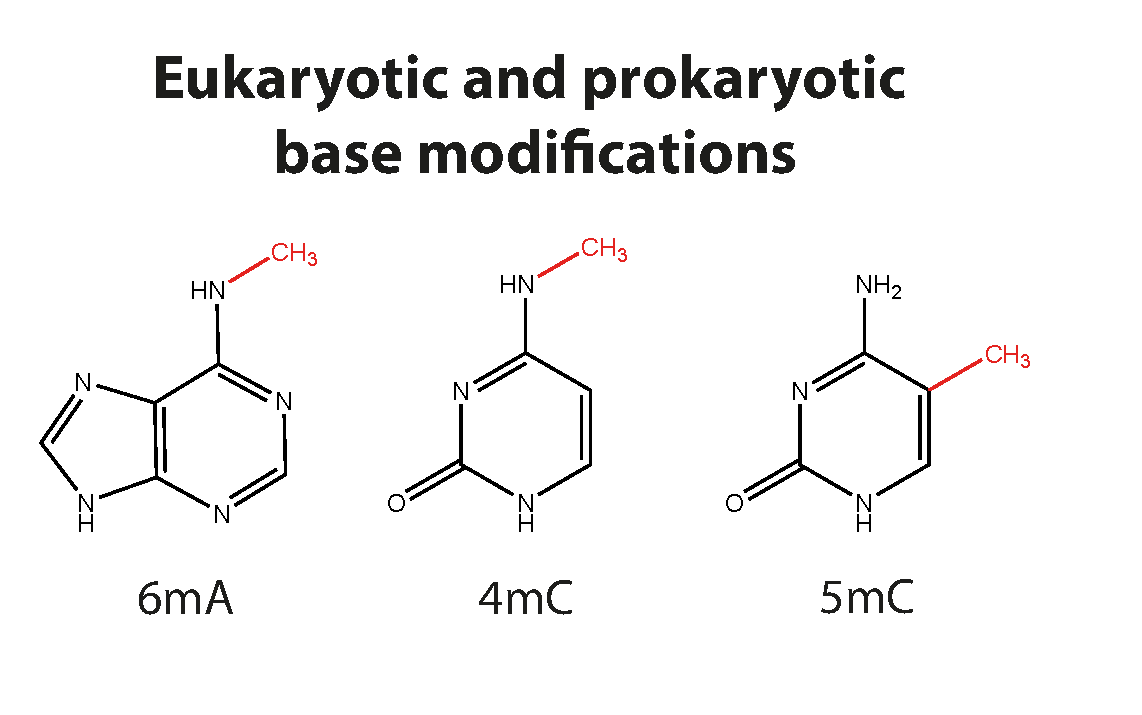
\includegraphics[width=0.5\textwidth]{Chapter1/Figs/base_mods.png}
\caption{}
\label{fig:meth_pathways}
\captionsetup{font=small}
    \caption*{}
\end{figure}

In eukaryotic systems including plants and animals DNA methylation works the other way around: The invading transposable elements are silenced by DNA methylation. DNA methylation can block transcription and gene expression directly by interfering with the binding of transcription factors. One of the earliest evidences for epigenetic modifications in plants was discovered in the \textit{Arabidopsis thaliana} gene SUPERMAN. Mutations in SUPERMAN affect normal floral development. Some alleles were discovered that had the mutant phenotype but an unchanged DNA sequence. The \textit{clark kent} epialleles were uncovered when it was discovered that the promoter sequence of SUP was methylated. In addition, SUP expression correlates with the extent of SUP promoter methylation \citep{RN100}.

\begin{figure}[htbp!] 
\centering    
    \includegraphics[width=1\textwidth]{Chapter1/Figs/RdDM.png}
\caption{}
\label{fig:RdDM_overview}
\captionsetup{font=small}
    \caption*{}
\end{figure}




DNA methylation also enters a self-reinforcing loop through RNA-directed DNA methylation (RdDM) and feeds into other silencing pathways including the recruitment of repressive histone modifications such as H3K9 methylation \citep{RN206,RN98,RN99}. The pattern of DNA modifications and therefore the expression pattern is inherited stably through mitosis. 

\section{Transposable elements} %Section - 1.2

The size of different plant genomes is highly variable and not necessarily related to their complexity. The largest eukaryotic genome size variation is 2400-fold, which can be found in flowering plants (e.g. \textit{Genlisea aurea}  63.6 Mb vs \textit{Paris japonica} 150 Gb \citep{RN76,RN81}). Transposable elements (TE) are selfish, repetitive DNA sequences that persist by inserting copies of themselves into various genomic locations \citep{RN102}. TEs are essential for driving genome evolution:  they can regulate gene expression, unequal crossover, recombination rate and in general contribute to genomic variation. TEs have had some prominent stabilising impacts on  chromosomes, playing a vital role in the evolution  of repetitive structures including the centromere  and telomeres \citep{RN101}, however the majority of TE  activity can cause harm to the genome and so is unfavourable to the organism \citep{RN103}.

Transposable elements can cause heritable disruption to a vast range of cellular functions by insertion into promoter, regulatory or genic regions. For example, the mobilisation of the CAC1 TE resulted in the disruption of the DWF4 gene and severe growth defects in Arabidopsis.

TEs are categorized into two classes: Class I (retrotransposons) and Class II (DNA transposons) TEs. Class I TEs are transcribed via an RNA intermediate, which then undergoes reverse transcription before insertion at another site in the genome. The reverse transcriptase necessary for this process is usually encoded within the transposable element coding sequence. One of the largest families of Class I TEs is long-terminal-repeat (LTR) retrotransposons. Some of these LTRs (flanking the TE) have picked up transfer-RNA (tRNA) fragments, which can be used as binding sites for host tRNAs. Subsequently, the clover leaf structure of the tRNA can be recognised as a primer to initiate reverse transcription and transposition. To combat this, some hosts cleave some tRNAs into tRNA fragments (tRFs) that compete for these LTR binding sites, thereby silencing these retrotransposons \citep{RN66,RN67,RN68}.

Conversely, class II TEs transcribe transposase enzymes that cut out and insert the DNA sections elsewhere in the genome. TEs from both classes can be further categorised into autonomous and non-autonomous elements, of which the former encodes all factors necessary for TE mobilisation and the latter does not, so transposition in this case is therefore dependent on trans-acting transposases \citep{RN106,RN107}.

As well as disturbing the function of individual genes, the process of excision and insertion of transposable elements can also destabilise genome structure \citep{RN103}. The repetitive nature of TEs can cause non-allelic homologous recombination during meiosis leading to reproductive defects and dicentric or acentric chromosomes \citep{RN108}. The contribution of TEs to genome size varies massively: whereas they comprise only ~21\% of the \textit{Arabidopsis thaliana} genome \citep{RN109},  crops with larger genomes have gone through significant TE amplification comprising of generally a few dominant TE families \citep{RN110,RN113}, resulting in a ~82\% and ~85\% genomic TE content of wheat and maize respectively \citep{RN110,RN111}. Consequently, the disruption of DDM1 in maize, a key chromatin remodeler involved in the genome wide maintenance of DNA methylation, results in embryo lethality \citep{RN112}. Therefore, whilst mutations of the components of the pathway for establishment and maintenance of DNA methylation have no apparent phenotypic effects in \textit{Arabidopsis thaliana}, it offers an important model system for exploring the underlying mechanisms of genome-wide epigenetic regulation.

\subsection{Classification, mechanism of transposition}
\subsection{TEs driving genome evolution}
\subsection{RNA-directed DNA methylation}

\section{Chromatin/histone modifications} %Section - 1.3

\section{DNA methylation maintenance and the RdDM pathway} %Section - 1.4

The existence of epigenetic marks implies that there are mechanisms to read, write and erase them. Cytosine methylation exists in one of three sequence contexts: CG, CHG or CHH (where H = A, T or C).  This contrasts with mammals in  which most methylation is directed to CG sites  and is not inherited by the next generation \citep{RN228}. 

RdDM is a pathway that can methylate cytosine regardless of the sequence context. In addition, in plants this is the only pathway through which de novo methylation is added to previously unmethylated regions. During DNA replication, DNA modifications at symmetric CG and CHG sites result in a hemimethylated state, whereby the daughter strands retain one methylated strand. A fully methylated state can be re-established through the highly conserved maintenance methyltransferases METHYLTRANSFERASE 1 (MET1, Dnmt1 homolog) and CHROMOMETHYLASE 3 (CMT3) (Fig. 1). CHH sites are maintained by CMT2, however, due to the asymmetry of the CHH modification, during replication, methylation information may be lost and RdDM is recruited for de novo methylation and maintenance. Therefore, to sustainably combat the detrimental effects of TE mobilisation, plants have evolved ways to keep transposon activity tightly controlled through RdDM.

It must be added that the robustness of the system is increased by the fact that CMT2/3 and SET domain histone methyltransferases (KYP, SUVH5/6) maintain non-CG methylation and H3K9me2 interdependently (namely, the chromo and the BAH domain of CMT3 interacts directly with H3K9me2 therefore having the ability to read other heterochromatic marks, establishing a positive feedback loop \citep{RN33}.

Following  the sequencing of the Arabidopsis genome, two new unexpected RNA polymerase II variants were found27 (RNA Polymerase IV and V). Through these two variants, the RdDM pathway generates small RNAs in heterochromatic regions and is able to target de novo DNA methylation to these regions. 
The RNA polymerase IV (Pol IV) associated pathway initiates through recruitment via H3K9me2 associated chromatin remodeller SAWADEE HOMEODOMAIN HOMOLOG 1 (SHH1) \citep{RN116}. Pol IV associates with chromatin remodellers CLASSY 1-4 (CLSY 1-4) and it transcribes a short single stranded precursor \citep{RN117} that is extended into double stranded RNA via RNA-dependent RNA polymerase 2 or 6 (RDR2 or RDR6)1,3. DICER LIKE 3 (DCL3) processes this transcript into 24 nucleotide small interfering RNAs (24nt siRNAs) which are loaded onto specific Argonaute proteins (AGO4/5/6/9)3 (Fig. 2).

Independently, RNA polymerase V (Pol V) is recruited by the DDR complex (chromatin remodellers DMS3, DRD1 and RDM1) and SUVH4/5/6 methyl-DNA-binding proteins, where it produces a single stranded transcript RNA scaffold \citep{RN33}. The siRNA-AGO complex binds to the complementary scaffold RNA and the AGO hook motif of the Pol V associated SPT5L protein in turn binds to AGO4. NRPE1 (a subunit of Pol V) and the de novo methyltransferase DRM2 associate with AGO4 and catalyse DNA methylation (Fig. 2)  \citep{RN228,RN121,RN122}. As discussed before, the maintenance of CHH sites therefore relies on persistent de novo methylation by DRM2.

Recently, it was shown that the CLASSY (CLSY) family of chromatin remodelling factors regulate tissue specific DNA methylation in \textit{Arabidopsis thaliana}, chiefly through the RdDM pathway. MethylC sequencing and sRNA sequencing in a variety of somatic and germline tissues revealed unique profiles of small RNAs and DNA methylation driven by specific CLSY expression profiles. This provides a model where unique expression profiles of chromatin remodellers define tissue-specific DNA methylation \citep{RN162}.  

Other key proteins involved in sRNA pathways during reproduction are ARGONAUTE (AGO) proteins. A group has recently discovered that during male meiosis, AGO1, AGO2 and AGO5 (involved in PGTS) were found in either the nucleus or cytoplasm, whilst AGO4 and AGO9 (involved in TGS) were found only in the nucleus. They also give an overview of the expression and localisation of several AGOs throughout meiosis, highlighting the dynamic expression and importance of these proteins through germline development. Additionally, they reveal that AGO1 and AGO5 binding miRNAs were present in meiocytes, suggesting that the miRNA pathway may be involved during meiosis \citep{RN149}.

Similarly, in sorghum, miRNAs were discovered to be differentially expressed before and after meiosis \citep{RN150}. In Arabidopsis, cucumber and soybean, several miRNAs were also found to be conserved and preferentially expressed in meiocytes although an overall lower abundance was observed when compared to soma \citep{RN151}.

In rice, another argonaute OsAGO18 was found to be specifically expressed in the meiocyte, and was involved in the accumulation of miRNA-triggered secondary siRNAs and the regulation of several pollen grain development genes \citep{RN153}. Additionally, it was also shown that the maintenance of CHH methylation through RdDM (specifically RDR2 which is a crucial component of the RdDM pathway), is required for both male and female sexual development in rice \citep{RN154}. It was also discovered that rice sporogenesis is dependent on the degradation of the germline-specific argonaute MEL1, preventing off-target effects of rogue phasiRNAs, which led to a semi-sterile phenotype \citep{RN155}.


\subsection{DNA modifications in plants, animals and prokaryotes}
\subsection{DNA methylation sequence contexts and their regulation in eukaryotes}
\subsection{AN overview of the RdDM pathway}

\section{Epigenetic reprogramming in plant sexual reproduction} %Section - 1.5
\subsection{RNA-directed DNA methylation and small RNAs}

In mammals, primordial germ cells are sequestered early in development and go through genome-wide demethylation during development and following fertilisation. This results in the resetting of global epigenetic marks as well as restoring pluripotency \citep{RN210}. Subsequent de novo re-methylation is mediated by methyltransferase Dnmt3 as well as germline specific PIWI-interacting small RNAs (piRNAs). The loss of the piRNA pathway results in transposon mobilisation, erroneous transcription regulation and reduction of fertility \citep{RN124,RN125,RN126}.

In the male lineage of angiosperms, the germline initiates from totipotent cells in the shoot apical meristem, giving rise to a diploid meiocyte. The meiocyte, surrounded by a layer of somatic nurse cells (the tapetum), undergoes meiosis, giving rise to a tetrad of microspores. The four microspores subsequently undergo mitotic division, to each make a vegetative cell (the somatic companion) and a generative cell which divides further to make two sperm cells (Fig. 3). 

Similarly to the tapetal nurse cell derived small RNAs catalysing DNA methylation in the male meiocyte, in the female germline, the surrounding somatic tissue synthesises RNA polymerase IV dependent 24 nucleotide small RNAs from (siren) loci \citep{RN164,RN163,RN162}. As well as nurse cell derived small RNAs, siren loci derived sRNAs are also CLSY3 and CLSY4 dependent \citep{RN162}, however there is little overlap between these two sets of loci and in fact between siren loci of different species \citep{RN163}. Despite their distinct origins, in Brassica rapa, siren loci derived sRNAs also catalyse DNA methylation largely at protein coding genes and regulating gene expression in the ovule \citep{RN165}. 

Further, it has been recently shown that 24 nucleotide small RNAs accumulate in rice zygotes, which overlap gene rich, distinct loci from paternally derived siRNA loci \citep{RN166}, highlighting the conserved nature of 24 nucleotide sRNA driven DNA methylation reprogramming in both the male and female sexual lineage. The importance of RdDM in embryonic development is further underpinned by a recent study that showed embryos resulting from a maternal RdDM mutant cross result in incorrect gene expression in the endosperm and a reduction in seed viability \citep{RN167}.

\begin{landscape}
\begin{figure}[htbp!] 
\centering    
    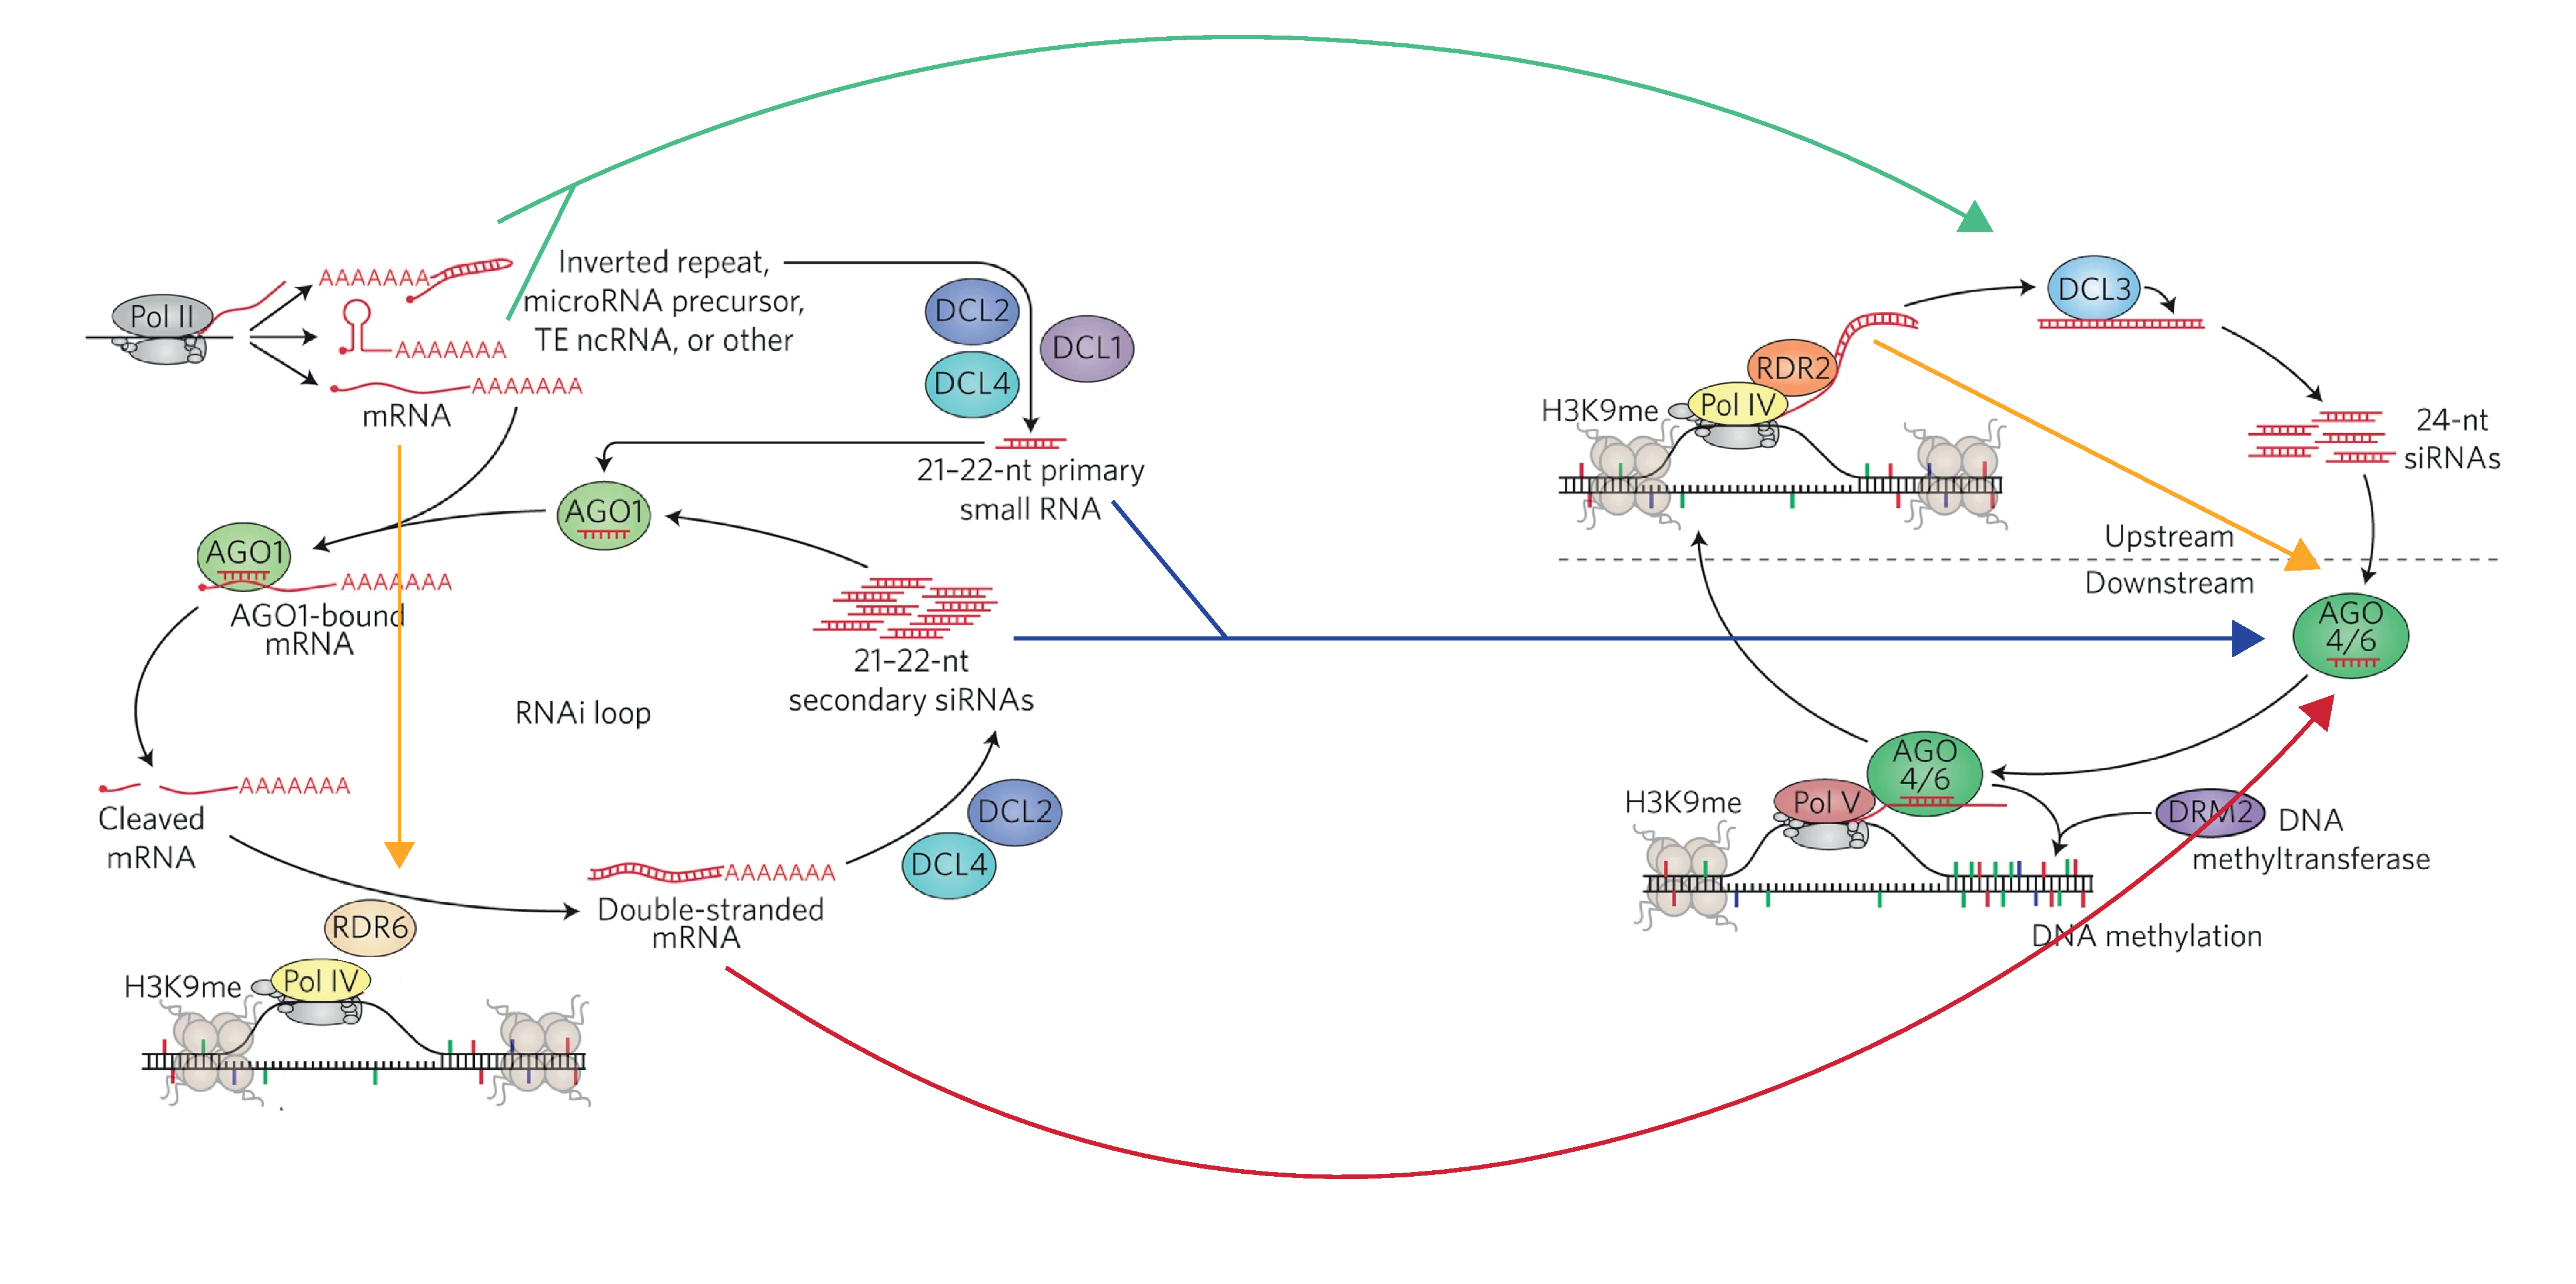
\includegraphics[width=1.5\textwidth]{Chapter1/Figs/ncRdDM.pdf}
\caption{}
\label{fig:ncRdDM}
\captionsetup{font=small}
    \caption*{}
\end{figure}
\end{landscape}



\subsubsection{In angiosperms}
\subsubsection{In Marchantia}
\subsection{Chromatin/histone modifications in reproduction}

\section{Thesis outline} %Section 1.6

It was previously thought that DNA methylation largely remained stable across reproductive cells in plants, due to its close association with the regulation of transposon activity \citep{RN247} and therefore genome integrity. Global demethylation does occur in companion cells of the germline, however, via passive or active demethylation. The former is due to decreased expression of MET1, leading to a lack of maintenance of methylation during DNA replication in the central cell. The latter is due to active demethylation by DEMETER (DME), which demethylates CG sites in the vegetative nucleus \citep{RN235,RN57}. This leads to the synthesis of 21nt epigenetically active small interfering RNAs (easiRNAs) in the vegetative cell from typically silenced TEs. As the vegetative cell is a terminal tissue rather than part of the germline, the destabilising effects to the genome is not of evolutionary concern. The easiRNAs produced from the vegetative cells move into the sperm cells where they accumulate and silence complementary target DNA sites through RdDM \citep{RN14,RN16}.

The RdDM pathway provides some of the essential communication between different cell types in reproductive tissue. AGO6 and AGO9 are a close paralog of AGO4 expressed in reproductive cells, which binds to 24nt RNA to direct RdDM. AGO6 is expressed in the shoot apical meristem, and there is increasing evidence that 21-22 nt secondary siRNAs (deriving from the miRNA pathway) can associate with AGO6 and participate in RdDM \citep{RN133,RN61,RN33}. Arabidopsis ago9 produces multiple megaspore mother cells (MMCs) in the female germline. Here, AGO9 is in the surrounding somatic nucellar cells, suggesting that sRNAs and corresponding essential RdDM machinery are transferred between cells.  TEs that are constitutively silenced in wildtype plants were reactivated in ago9 embryo sacs, suggesting a pathway similar to the mammalian piRNA pathway previously discussed \citep{RN14}.

Recent work identified male sexual lineage specific DNA methylation reprogramming in the Arabidopsis germline. In general, male meiocytes maintain high levels of CG and CHG methylation when compared to somatic canonical RdDM loci levels, and a relatively low level of CHH methylation. However, in the CHH context, there is distinct hypermethylation at selected, sexual lineage specific loci (HyperTEs), including novel targets of RdDM activity. Further, de novo gene associated methylated loci were also identified (MetGenes), including a meiosis specific gene \citep{RN199}.

Further, it was discovered that meiocytes themselves are quiescent in sRNA biogenesis. The biogenesis of these germline specific siRNAs is in the somatic tapetal tissue and is associated with the chromatin remodeller CLASSY3. Nurse cell-derived siRNAs are then transported into the meiocyte from the tapetum, inducing DNA methylation at HyperTE loci. MetGene loci can be uniquely targeted for methylation in the meiocyte by imperfectly matching siRNA derived from HyperTEs. These nurse-cell derived siRNAs inform the entire male sexual lineage specific methylation reprogramming, from meiocyte to sperm \citep{RN187}.

The mechanism of movement of sRNA between companion and germline cells needs more evidence, however there is extensive evidence of cross-cellular RNA movement. Plasmodesmata provide a cytoplasmic network between cells (such as the tapetum and meiocyte) which allows nutrient transport but have also been shown to allow RNA movement between cells \citep{RN130,RN132,RN128}.

The aim of this project is to shed light on the mechanism by which this germline specific sRNA and DNA methylation profile is established. Namely, to investigate the sRNA profiles of the microspore, vegetative and sperm cells, and to examine the key factors involved at each step (e.g. CLASSY chromatin remodelers, specific Argonautes).  

The field of small RNA biology in germlines is still rapidly evolving so here is a summary of a number of key findings since last year. For a detailed introduction to small RNAs in plant germlines, please refer to my second-year review and probation review.

Similarly to the tapetal nurse cell derived small RNAs catalysing DNA methylation in the male meiocyte, in the female germline, the surrounding somatic tissue synthesises RNA polymerase IV dependent 24 nucleotide small RNAs from (siren) loci2-4. As well as nurse cell derived small RNAs, siren loci derived sRNAs are also CLSY3 and CLSY4 dependent4, however there is little overlap between these two sets of loci and in fact between siren loci of different species3. Despite their distinct origins, in Brassica rapa, siren loci derived sRNAs also catalyse DNA methylation largely at protein coding genes and regulating gene expression in the ovule5. 

Further, it has been recently shown that 24 nucleotide small RNAs accumulate in rice zygotes, which overlap gene rich, distinct loci from paternally derived siRNA loci6, highlighting the conserved nature of 24 nucleotide sRNA driven DNA methylation reprogramming in both the male and female sexual lineage. The importance of RdDM in embryonic development is further underpinned by a recent study that showed embryos resulting from a maternal RdDM mutant cross result in incorrect gene expression in the endosperm and a reduction in seed viability7.
